% Intended LaTeX compiler: pdflatex
\documentclass[10pt,a4paper,UTF8]{article}
\usepackage{zclorg}
\usepackage{tikztheorem}
\author{zcl.space}
\date{}
\title{Functions and Maps}
\hypersetup{
 pdfauthor={zcl.space},
 pdftitle={Functions and Maps},
 pdfkeywords={PMA},
 pdfsubject={},
 pdfcreator={Emacs 25.0.50.1 (Org mode 9.1.2)},
 pdflang={English}}
\begin{document}

\maketitle
\tableofcontents
\titlepic{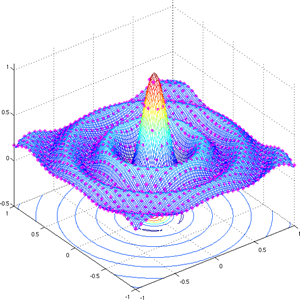
\includegraphics[scale=0.25]{../../img/sinc.PNG}}

\section{Sets}
\label{sec:org024cc21}
A set \(A\) divides the mathematical universe into two parts:
those objects \(x\) that \textbf{belong} to \(A\) and those that don't.
The notation \(x\in A\) means \(x\) belongs to \(A\).
The notation \(x\notin A\) means that \(x\) does not belong to \(A\).
The objects that belong to \(A\) are sometimes called
the \textbf{elements} of \(A\) but we will often call them \textbf{points}
or \textbf{numbers}.
Other words  roughly synonymous with the word \textbf{set}
are \textbf{class} , \textbf{collection} , and \textbf{aggregate} .
These longer words are generally used to avoid
using the word \textbf{set}  twice in one sentence.  The situation typically
arises when an author wants to talk about sets whose elements are themselves
sets. One  might write ``the collection of all finite sets of integers'',
rather than ``the set of all finite sets of integers''.

For two sets \(A\) and \(B\),   the notation \(A\subseteq B\) means that \(A\) is a \textbf{subset}
of \(B\), i.e. for all \(x\) we have \(x\in A\implies x\in B\).
By definition, two sets are \textbf{equal} if each is a subset of the other:
$$
   A=B\iff A\subseteq B\mbox{ and } B\subseteq A.
$$
The notation \(\{x:P(x)\}\) denotes the set of all \(x\)
for which  the property \(P(x)\) is  true.
The notation \(\{x\in A:P(x)\}\) denotes the set of all \(x\in A\)
for which  the property \(P(x)\) is  true.
Finite sets may be defined by enumerating their elements as in
$$
   x\in\{a_1,a_2,\ldots,a_n\}\iff x=a_1 \mbox{ or } x=a_2 \mbox{ or } \cdots \mbox{ or } x=a_n
$$
and often infinite sets as well as in
$$
    \mathbb{N}=\{0,1,2,\ldots\}, \qquad \mathbb{Z}=\{\ldots,-2, -1,0,1,2,\ldots\},\qquad \mathbb{Z}^+=\{1,2,3,\ldots,\}.
$$

If \(A\) and \(B\) are sets, then
the sets
$$
   A\cup B:=\{x: x\in A\mbox{ or } x\in B\},\qquad
   A\cap B:=\{x: x\in A\mbox{ and } x\in B\},
$$
are called respectively the \textbf{union} and \textbf{intersection}  of \(A\) and \(B\).
The \textbf{empty set}  is denoted \(\emptyset\):  For all \(x\) it is true that
$$
x\notin\emptyset.
$$
Two sets are \textbf{disjoint}  iff they have no elements in common, i.e
iff \(A\cap B=\emptyset\). The set
$$
   X\setminus A:=\{x\in X: x\notin A\}
$$
is called the \textbf{complement}  of \(A\) in \(X\).\footnote\{
Morgan uses the notation \$A\^{}\complement \$ for \(\mathbb{R}^n\setminus A\) (when \(A\) is a subset of \(\mathbb{R}^n\)).
\}
The set
$$
   A\times B:=\{(x,y): x\in A\mbox{ and } y\in B\}
$$
of all ordered pairs \((x,y)\) with \(x\in A\) and \(y\in B\) is called the \textbf{Cartesian product}
of \(A\) and \(B\). The term \textbf{direct product}  is a synonym. We also use the notation
$$
     A^n:= \underbrace{A\times A\times \cdots\times A}_n
$$
In particular,
$$
\mathbb{R}^n :=\{(x_1,x_2,\ldots,x_n): x_i\in\mathbb{R}\}
$$
 denotes the vector space of all \$n\$tuples of real numbers,
so \(\mathbb{R}^1=\mathbb{R}\), \(\mathbb{R}^2= \mathbb{R}\times \mathbb{R}\), \(\mathbb{R}^3=\mathbb{R}\times \mathbb{R}\times \mathbb{R}\), etc.\footnote\{
Buck uses  the term \textbf{\(n\) space}  as a synonym for \(\mathbb{R}^n\).\}


 Do not confuse an \textbf{\$n\$tuple}  (finite sequence of length \(n\)) with a finite set.
For the former order is important:  \(\{3,7\}=\{7,3\}\)  but \((3,7)\ne(7,3)\);
for the latter repetitions don't matter: \(\{2,2,3\}=\{2,3\}\) but \((2,2,3)\ne(2,3)\).

An \textbf{indexed family of sets}  is a function which assigns
a set \(A_i\) to each element \(i\) of a set \(I\).
The set \(I\) is called the \textbf{index set}  of the family and
the family is usually denoted \((A_i)_{i\in I}\).
The \textbf{union}  and \textbf{intersection}  of the indexed family are defined by
\begin{eqnarray*}
  x\in \bigcup_{i\in I} A_i &\iff& \exists i\in I\;\mbox{such that}\; x\in A_i.\\
  x\in \bigcap_{i\in I} A_i &\iff& \forall i\in I\;\mbox{we have}\; x\in A_i.
\end{eqnarray*}
The notation \(\exists i\in I\) is an abbreviation for ``there exists \(i\in I\)'', and
the notation \(\forall i\in I\) is an abbreviation for ``for all \(i\in I\)''.
In these definitions the set \(I\) can be infinite.
For finite sets \(I\) we recover the earlier definitions, e.g.
for \(I=\{1,2\}\) we have
$$
\bigcup_{i\in\{1,2\}} A_i=A_1\cup A_2 ,\qquad \bigcap_{i\in\{1,2\}} A_i=A_1\cap A_2.
$$
This illustrates the logical principle that \(\exists\) is like an ``infinite or'' and
\(\forall\) is like an ``infinite and''.


\rmk\label{rmk:truth_table} Set theory is simply a way of formalizing logic.
Simple set theoretic identities may be proved by *truth tables\}.
For example, consider the following ``distributive law''
$$
     (A\cup B)\cap C = (A\cap C)\cup(B\cap C).
$$
To show that \(x\in(A\cup B)\cap C \iff x\in(A\cap C)\cup(B\cap C)\) we can simply consider all the possibilities:

\begin{array}{ccc|cc}
A&B&C& (A\cup B)\cap C & (A\cap C)\cup (B\cup C)\\ \hline
T&T&T&               T            &                    T\\
T&T&F&               F            &                    F\\
T&F&T&               T            &                    T\\
T&F&F&               F            &                    F\\
F&T&T&               T            &                    T\\
F&T&F&               F            &                    F\\
F&F&T&               F            &                    F\\
F&F&F&               F            &                    F
\end{array}

It is usually not necessary to show so much detail in your written work,
but it will be hard for you to decide just how much detail \textbf{is}  appropriate.
A good rule of thumb is that you should be prepared to supply more detail if challenged.


From logic we know that
$$
\mathrm{not }\;\exists \iff \forall\;\mathrm{ not},
\qquad \mbox{ and } \qquad
\mathrm{not }\;\forall \iff \exists\; \mathrm{ not},
$$
 so
for any set \(X\) and any indexed family \((A_i)_{i\in I}\) we have
$$
  X\setminus \bigcup_{i\in I} A_i = \bigcap_{i\in I} (X\setminus A_i),
  \qquad
  X\setminus \bigcap_{i\in I} A_i = \bigcup_{i\in I} (X\setminus A_i).
$$
Logicians call these  \textbf{De Morgan's Laws} . In particular, for \(I=\{1,2\}\) we have
\begin{aligned}
& X\setminus(A_1\cup A_2)= (X\setminus A_1)\cap(X\setminus A_2),
  \\
& X \setminus(A_1\cap A_2)= (X \setminus A_1)\cup(X \setminus A_2).
\end{aligned}

Also by logic we have set theoretic distributive laws
$$
  X\cap \bigcup_{i\in I} A_i = \bigcup_{i\in I} (X\cap A_i),
  \qquad
  X\cup\bigcap_{i\in I} A_i = \bigcap_{i\in I} (X\cup A_i).
$$
In particular, for \(I=\{1,2\}\) we have

\begin{aligned}
&X\cup(A_1\cap A_2)= (X\cup A_1)\cap(X\cup A_2),
  \\
&X\cap(A_1\cup A_2)= (X\cap A_1)\cup(X\cap A_2).
\end{aligned}




\section{functions and maps}
\label{sec:org4257448}
 A \texttt{function} is a rule which assigns a value
\(f(x)\) to every point \(x\) from a set called the \texttt{domain} of the function.
The set
$$
  \mathrm{graph}(f):=\{(x,y): y=f(x)\}
$$
of all pairs \((x,y)\) such that \(y=f(x)\) is called the \texttt{graph} of the function \(f\).
Two functions are equal iff they have the same graph.

Let \(X\) and \(Y\) be sets.
We say that \(f\) is a \texttt{map}  from \(X\) to \(Y\)
and  write \(f:X\to Y\) when \(f\) is a function which assigns
a point \(y=f(x)\in Y\) to each point \(x\in X\).
Two maps \(f:X\to Y\) and \(f':X'\to Y'\) are
said to be \texttt{equal}
when \(X=X'\), \(Y=Y'\), and \(f(x)=f'(x)\) for all \(x\in X\).
Thus if \(f\) and \(f'\) equal maps, then \(\mathrm{graph}(f)=\mathrm{graph}(f')\)
but not conversely (because \(Y=Y'\) is part of the definition of equality for maps).
However most authors would say that two functions are equal iff they have the same graph.

 Some authors
use the notation \(x\mapsto f(x)\)
to define a map. This allows them to avoid introducing a name for the map. Thus instead of writing
\begin{quote}
Consider the map \(f:\mathbf{R}\to \mathbf{R}\) defined by \(f(x)=x^5+x\).
\end{quote}

they may write
\begin{quote}
Consider the map \(\mathbf{R}\to \mathbf{R}:x\mapsto x^5+x\).
\end{quote}

When \(A\subseteq X\), \(B\subseteq Y\), and \(f:X\to Y\), the sets

\begin{aligned}
  & f(A):=\{y\in Y: \exists x\in A \mbox{ such that }y=f(x)\}, \\
  & f^{-1}(B):=\{x\in X: f(x)\in B\},
\end{aligned}

are called respectively the \texttt{image} of \(A\)  by \(f\)
and  \texttt{inverse image}  of \(B\) by \(f\).

The sets \(X\)  and \(Y\) are sometimes called the
\texttt{source} and \texttt{target} of a map \(f:X\to Y\).
The image \(f(X)\) of the source is what is called the \{range\}
of the function \(f\) in calculus.
Thus the domain of a map is the same as its source
while the range is a subset of its target.

There are slight variations in terminology among  authors.
Morgan avoids the word \texttt{map} and Lang sometimes
uses the word \texttt{mapping}.  Buck uses the term the \texttt{preimage}
instead of \texttt{inverse image}. Lang  uses the \(\mapsto\)
notation but the other authors apparently avoid it.
For Lang a function is a map whose target is \(\mathbf{R}\).
In precalculus courses a function is usually defined by an expression
and the domain is implicitly taken to be the largest set of numbers
for which the expression is meaningful, but in advanced mathematics
authors usually make the domain explicit.
\end{document}
